\chapter{Demonstrativ- vs. Definitartikel}\label{chap:demdef}

Ein Ziel der vorliegenden Arbeit ist, das funktionale Spektrum von ahd. \object{dër} systematisch zu erfassen. Hierzu braucht man Kriterien, die es ermöglichen, De"-mon"-stra"-tiv- von Definitartikeln theoretisch und empirisch  abzugrenzen. In diesem Kapitel wird auf Basis der Forschung eine Typologie von Gebrauchskontexten zusammengestellt, die typisch für die beiden Artikelarten sind. Nach einem kurzen Überblick über die wichtigsten Ansätze zur semantischen Analyse definiter Ausdrücke in Abschnitt \ref{sec:definitheitstheorien} führt Abschnitt \ref{sec:demonstrativartikel} in typische Gebrauchskontexte für Demonstrativartikel ein. Davon abgrenzend listet Teil \ref{sec:definitartikel} die Kontexte auf, in denen Definitartikel vorkommen. In Abschnitt \ref{sec:pragsem} wird das  Löbnersche Konzept der pragmatischen und semantischen Definita vorgestellt, das sich insbesondere in der historischen Sprachwissenschaft etabliert hat, um Demonstrativ- von Definitartikel zu unterscheiden. 

\section{Semantische Analysen definiter Ausdrücke} \label{sec:definitheitstheorien}

Der Definitartikel gilt als prototypischer Ausdruck der grammatischen Kategorie Definitheit. Die Frage, was genau unter Definitheit zu verstehen ist bzw. welche Funktion dem Definitartikel als Vertreter dieser Kategorie innewohnt, ist viel diskutiert und unterschiedlich beantwortet worden \parencite[zum Überblick  s.][]{Bisle-Muller1991,Hauenschild1993,Lyons1999,Abbott2007,Cui2014}.

So ist für die formale Semantik bis heute Russels Einzig"-artig"-keits-Prä"-supposi"-tion (\object{unique"-ness}) relevant, um definite von indefiniten Ausdrücken abzugrenzen (\cite{Russel1905}, vgl. weiterführend \cite{Heim1991,Heim2011}). Es handelt sich hierbei um einen Beschreibungsansatz, der NPs, die genau einen Referenten denotieren, wie z.B. Unika (\object{die Sonne}) oder Superlative (\object{der beste Vortrag}) besonders gut erfassen kann; für  Plural-NPs  ist er allerdings problematisch \parencite[vgl. die Diskussion hierzu in][7--11] {Lyons1999}. \textcite{Hawkins1978} liefert eine Abwandlung dieses Konzepts, in dem er statt \object{unique"-ness} die \object{inclusiveness} definiter Ausdrücke postuliert \parencite[kritisch hierzu:][32]{Bisle-Muller1991}. Dahinter steht die Idee, dass mithilfe des Definitartikels auf die Gesamtheit aller Referenten, die der definiten Beschreibung genügen, Bezug genommen wird.

Ein weiterer viel zitierter und pragmatisch ausgerichteter Ansatz stammt von \textcite{Christophersen1939}. Demnach können definite NPs nur dann richtig verstanden werden, wenn sowohl der Sprecher als auch der Hörer den Referenten als bekannt einstufen. Diese \object{familarity}-Theorie kann allerdings allen nicht anaphorisch gebrauchten Verwendungen des Definitartikels kaum standhalten wie u.a. \textcite{Hawkins1978} und \textcite{Lobner1985} zeigen. Aufbauend auf \textcite{Lewis1970} versucht \textcite{vonHeusinger1996} den Problemen der traditionellen Definitheitstheorien beizukommen, indem er Definitheit mit \object{Salienz} in Verbindung bringt: Definite Ausdrücke beziehen sich demnach immer auf den salientesten Referenten im Diskurs. Dieser Ansatz ist zwar für anaphorische und situativ-gebrauchte Definita nützlich, stößt allerdings beim sog. assoziativ-anaphorischen Gebrauchskontext an Grenzen \parencite[s. auch][144--149]{Cui2014}, da hier der Referent erst über einen Assoziationsprozess aktiviert werden muss und damit gerade keine hohe Salienz aufweist (s. Abschnitt \ref{sec:asso}).

In der historischen Sprachwissenschaft hat sich das Definitheitskonzept von \textcite{Lobner1985} etabliert, um Demonstrativ- und Definitartikel funktional voneinander abzugrenzen \parencite{Demske2001,Szczepaniak2011a,Schlachter2015}. Hierbei wird zwischen pragmatischer und semantischer Definitheit unterschieden; letztere entspricht der Domäne des Definitartikels (vgl. vertiefend hierzu Abschnitt \ref{sec:pragsem}). 

Den genannten  semantischen Analysen ist gemein, dass von bestimmten Gebrauchskontexten, die für den Definitartikel als typisch angesehen werden, ausgegangen wird \parencite[9]{Cui2014}. Meist steht dahinter das theoretische Ideal, dass sich aus diesen Kontexten \herkur{eine} bestimmte Basisfunktion für den Definitartikel erarbeiten lässt. Aus einer historischen Perspektive ist es ganz natürlich, dass eine sprachliche Form auch unterschiedliche Funktionen übernehmen kann und sich das Verhältnis von Ausdruck und Inhalt über die Zeit wandelt. In der vorliegenden Untersuchung geht es um die Frage, welches funktionale Spektrum das ahd. \object{dër} zu bestimmten Zeitpunkten in der Geschichte des Deutschen einnimmt. Konkret soll ermittelt werden, ob \object{dër} in den unterschiedlichen ahd. Überlieferungen als Demonstrativ- oder Definitartikel zu klassifizieren ist. Für die Beantwortung dieser Frage kann man sich die Gebrauchskontexte zunutze machen, die den beiden Artikeltypen in der Forschung zugesprochen werden. Sie sind Gegenstand der nächsten beiden Abschnitte. 


\section{Gebrauchskontexte für Demonstrativartikel}\label{sec:demonstrativartikel}

In allen Sprachen der Welt gibt es Demonstrativa, d.h. deiktische Ausdrücke, die auf außersprachliche Entitäten verweisen oder diskursintern Wissen (re)ak"-ti"-vieren \parencite{Diessel1999, Diessel2006}. Neben pronominalen (\object{Wusstest du \textbf{das}?}) und adverbial gebrauchten Demonstrativa (z.B. \object{hier}) unterscheidet man die Klasse der adnominalen Demonstrativa, also den Demonstrativartikeln (\object{Ich kaufe mir \textbf{dieses/jenes} Buch}), aus denen  Definitartikel typischerweise hervorgehen (s. ausführlich Kapitel \ref{chapter:theorie}). Es werden vier Kontexte unterschieden, in denen Demonstrativartikel auftreten: der situative, der anaphorische, der diskursdeiktische und der anamnestische Gebrauchskontext \parencite[s. u.a.][]{Hawkins1978,Lyons1979,Bisle-Muller1991,Himmelmann1996,Himmelmann1997,Fillmore1997,Diessel1999,Schwarz2000,Consten2004,Diessel2006,Diessel2012, Studler2011}. Diese lassen sich anknüpfend an die Terminologie von \textcite{Halliday1993} unter die Begriffspaare exophorisch (= situativ) und endophorisch (= nicht-situativ) fassen \parencite[vgl. auch][6]{Diessel1999}, zur Übersicht s. Abbildung \ref{abb:demonstrativa-gebrauchskontexte}. Für die Entwicklung des Definitartikels sind die endophorischen Kontexte (vor allem der anaphorische und der anamnestische Gebrauch) besonders relevant, da sie kategorielle Schnittstellen zum Definitartikel bilden (vgl. ausführlich die Diskussion in \ref{sec:bruecke}). In den nachfolgenden Abschnitten erfolgt die Diskussion der einzelnen Kontexte. 

\begin{figure}[h]
% 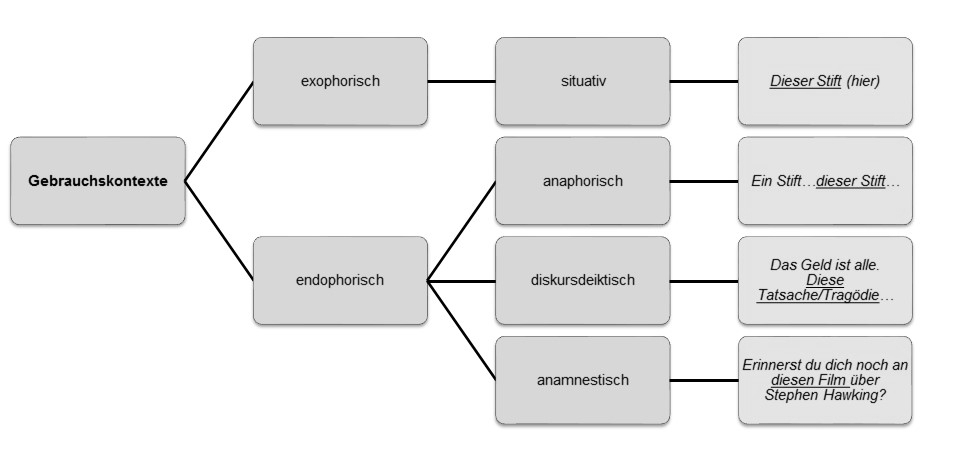
\includegraphics[width=12cm]{images/Gebrauchskontexte-demonstrativa-neu-sw.jpg}
\begin{forest}
for tree = {forked edges,grow'=east,anchor=east,minimum width=3cm,align=center,draw,s sep=\baselineskip}
[Gebrauchskontexte,rotate=90,anchor=north
  [exophorisch [ situativ,tier=isch [ \textit{\uline{Dieser Stift} (hier)} ] ] ]
  [endophorisch
    [anaphorisch,tier=isch [ \textit{Ein Stift\ldots\uline{dieser Stift}\ldots} ] ]
    [diskursdeiktisch,tier=isch [ \textit{Das Geld ist alle.}\\\textit{\uline{Diese Tatsache\slash Tragödie}\ldots} ] ]
    [anamnestisch,tier=isch [ \textit{Erinnerst du dich noch}\\\textit{an \uline{diesen Film} über}\\\textit{Stephen Hawking?} ] ]
  ]
]
\end{forest}
\caption {Gebrauchskontexte von Demonstrativa\label{abb:demonstrativa-gebrauchskontexte}}
\end{figure}



\subsection{Situativer Gebrauch}\label{sec:situativ}

Beim situativen Gebrauch \parencite[auch deiktischer Gebrauch, z.B. bei][]{Bisle-Muller1991,Consten2004,Studler2011} führt der Demonstrativartikel einen Referenten in das gemeinsame Diskursuniversum von Sprecher und Hörer ein, indem mit seiner Hilfe auf eine Entität in der unmittelbaren Äußerungssituation verwiesen wird, s. \REF{ex:deikt}. Zugleich erfolgt eine Verortung im Raum.

\begin{exe}
	\ex \label{ex:deikt} \object{\textbf{Dieser Stift} (hier) schreibt gut.}
\end{exe}

Proximale Demonstrativa kennzeichnen Entitäten, die dem Sprecher nahe sind, z.B. \object{dieser}, distale markieren Distanz, z.B. \object{jener, dieser/der da}.
%\footnote{Diese Zweigliedrigkeit ist in allen Sprachen der Welt gegeben; zu komplexeren Systemen s. \textcite[35--55]{Diessel1999}.} 
Damit das Referieren glückt, müssen die Diskursteilnehmer ihr Wissen mit der Perspektive des Sprechers, dem deiktischen Zentrum oder  \object{origo} \parencite{Buhler1934} abgleichen  \parencite[s. auch][327ff.]{Hoffmann2009}. Der Verweis kann mit einer Zeigegeste unterstützt werden; zu Ausnahmen und weniger zentralen Fällen des situativen Gebrauchs s. \textcite[S. 94f.]{Diessel1999} und \textcite[219--224]{Himmelmann1996}. 

Mit \textcite[]{Buhler1934} kann man den situativen Gebrauch in zwei Arten des Zeigens unterteilen. Bei der sog. \object{Demonstratio ad oculos} zielt die Zeigegeste auf einen Referenten, der in der unmittelbaren Umgebung vorhanden und somit für die Diskursteilnehmer sichtbar ist (typisch für die Face-to-Face-Kommunikation). Die sog. \object{Deixis am Phantasma} umfasst hingegen demonstrative Ausdrücke, die innerhalb der bloßen Vorstellung operieren: Der Referent wird zwar im Diskursuniversum verortet, ist aber nicht physisch anwesend \parencite[s. auch][222]{Himmelmann1996}. Dieser Gebrauch gilt für alle Kommunikationsformen, in denen Äußerungen zeitlich und räumlich vom Sprecher entkoppelt sind, also z.B. in narrativen Texten \parencite[95]{Diessel1999} oder auch in wissenschaftlichen Beschreibungen, in denen das deiktische Zentrum von einem imaginären Sprecher ausgeht. Der situative Gebrauch ist in diesem Sinne auch in Dokumenten aus älteren Sprachstufen zu erwarten. 

Mit der situativen Verortung -- sei sie konkret oder imaginär -- geht immer ein kognitiver Abgrenzungsprozess zu anderen potentiellen Referenten einher, etwa  \object{Ich möchte diesen (und nicht jenen) Stift} \parencite[vgl.][70]{Bisle-Muller1991}, wodurch der Referent eindeutig determiniert und identifiziert werden kann \parencite{Hoffmann2009}. 

 
\subsection{Anaphorischer Gebrauch}\label{sec:anaphorisch}

Während die eindeutige Determination beim situativen Gebrauch über den außersprachlichen Kontext gewährleistet wird, kommt beim anaphorischen Ge"-brauch die textuelle Umgebung ins Spiel\footnote{Die textuelle Umgebung schließt sowohl schriftliche als auch mündlich Diskurstypen ein.}, denn es wird auf einen zuvor im Diskurs etablierten Referenten verwiesen (den Antezedens), s. \REF{ex:anaph} \parencite[vgl.][229]{Himmelmann1996}.\footnote{In Opposition hierzu stehen \object{kataphorische} Ausdrücke: Sie sind koreferentiell mit nachfolgenden Referenten, welche erst im weiteren Diskursverlauf  hinreichend identifiziert werden können \parencite[s.][161f.]{Veldre-Gerner2007}. Beim vergleichsweise seltenen kataphorisch gebrauchten Demonstrativartikel kann eine pejorative Lesart mitschwingen (\object{Auf der Party war dieser Student. Er hieß John und...}). Zur Diskussion solcher Verwendungsweisen als möglichen Ausdruck von Spezifizität s. \textcite[533]{deMulder2011}.}

\begin{exe}
	\ex \label{ex:anaph} \object{Es war einmal ein König. \textbf{Dieser König} hatte drei Söhne...}
\end{exe}

Im Vergleich zu anderen Mitteln der Wiederaufnahme (Personalpronomen oder Definitartikel) zeichnen sich anaphorische Demonstrativartikel (und Demonstrativa allgemein) dadurch aus, dass sie eine (Neu-)Fokussierung von Referenten im Diskurs bewirken \parencite [s. u.a.][]{Ehlich1979,Prince1981,Gundel1993,Comrie1997,Himmelmann1996,Diessel1999,Kibrik2011}. Sie werden daher häufig gebraucht, um einen Topikwechsel zu vollziehen. In Beispiel \REF{ex:topic} \parencite[angelehnt an][96]{Diessel1999}, impliziert das Personalpronomen \object{er} Koreferentialität mit dem Topik \object{Anwalt}, während sich das Demonstrativum \object{der} nur auf \object{Klient} beziehen kann, der zu diesem Zeitpunkt zwar kognitiv aktiviert, aber nicht fokussiert und \blockcquote[96]{Diessel1999}{somewhat unexpected} ist \parencite[vgl. hierzu][278f.]{Gundel1993}. Im Gegensatz hierzu ist die Wiederaufnahme des bereits im Fokus stehenden \object{Anwalt} mit \object{dieser Anwalt} blockiert. Am natürlichsten erscheinen die pronominalen Wiederaufnahmen. Mit der Phrase \object{dieser Klient} kann allerdings besonders stark betont werden, dass jetzt der Klient und nicht -- wie erwartet -- der Anwalt im Mittelpunkt des weiteren Diskursverlaufs steht.   

\begin{exe}
	\ex \label{ex:topic} \object{Der Anwalt sprach mit einem Klienten. Da \textbf{er/der/dieser Klient/*dieser Anwalt} nur wenig Zeit hatte, vereinbarten sie ein weiteres Gespräch für die nächste Woche.} 
\end{exe}

Das Potential, einen Topikwechsel einzuleiten, lässt sich darauf zurückführen, dass es zur Hauptfunktion von Demonstrativa gehört, Referenten, die gerade neu eingeführt wurden, anaphorisch wiederaufzunehmen.\footnote{Vgl. hierzu auch die Studie zum Schwedischen von Fraurud, in der empirisch belegt wird, dass Demonstrativartikel fast ausschließlich anaphorisch gebraucht werden \parencite[400]{Fraurud1990}.} Dies gilt insbesondere für artikellose Sprachen  \parencite[229]{Himmelmann1996}, aber auch für Sprachen, die einen Definitartikel ausgebildet haben, etwa das Englische. Christophersen beobachtet \blockcquote[vgl.][29]{Christophersen1939} {a certain aversion to the use of a \object{the}-form immediately after the word is introduced; a demonstrative is more usual in such cases}. Demonstrativa sind also die erste Wahl, um ein Topik im Diskurs nach Ersterwähnung des Referenten zu etablieren. Für die  anschließende referentielle Kontinuität sorgen  Personalpronomen oder Definitartikel, indem sie das Topik im Fokus der Aufmerksamkeit halten. 

\subsection{Diskursdeiktischer Gebrauch}\label{diskurs-deikt}

Werden Demonstrativartikel zum Zwecke der Diskursdeixis eingesetzt, verweisen sie nicht auf einzelne NPs, sondern auf größere syntaktische Einheiten, also Sätze, Abschnitte oder Texte \parencite{Webber1991,Fraurud1992, Fillmore1997, Diessel1999, Consten2007, Consten2009, Marx2011}. Durch die anaphorische Wiederaufnahme werden die zuvor genannten Informationen zu einem abstrakten Referenten gebündelt (z.B. \object{Tatsache, Prozess, Zustand}) und können dann evaluierende Zusatzinformationen transportieren (\object{Ungerechtigkeit, Tragödie, Zufall})\footnote{\textcite{Schmid2000} bezeichnet diesen Nomentypus als  \object{shell-noun}.},  s.\ref{diskurs}.\footnote{Da dieser anaphorische Prozess die \blockcquote[129]{Schwarz2000}{kognitive Strategie der Komplexbildung} voraussetzt, hat sich in neueren Arbeiten zur Textlinguistik der Begriff \object{Komplex-Anaphern} etabliert \parencite[s. z.b.][]{Consten2007, Consten2009}. Einen Überblick über weitere terminologische Vorschläge der letzten Jahrzehnte bietet \textcite[16f.]{Marx2011}, zur Abgrenzung von Diskursdeixis und Anapher s. \textcite[30f.]{Consten2004}.} 

 \begin{exe}
	\ex \label{diskurs}  \object{Jedes Jahr sind tausende Menschen auf der Flucht.}
	\begin{xlist}
		\ex \label{propo} \object{\textbf{Diese Tatsache} lässt viele erschauern.}
			\ex \label{bewertung} \object{\textbf{Diese Ungerechtigkeit} muss behoben werden.}
		\end{xlist}
\end{exe}

Zwar kann der diskursdeiktische Gebrauch nur über einen anaphorischen Bezug gelingen, der eigentliche Referent wird allerdings erst zum Zeitpunkt des Verweises im Diskurs etabliert, wodurch die Diskursdeixis dem situativen Gebrauchskontext ähnelt \parencite[224]{Himmelmann1996}. Beide Kontexte fallen typischerweise in die Domäne von pro- oder adnominalen Demonstrativa; ein Austausch mit dem Definitartikel ist theoretisch möglich, aber markiert, vgl. \ref{def-diskurs} \parencite[Beispiele nach][130f.]{Schwarz2000}.  

 \begin{exe}
	\ex \label{def-diskurs} 
	\begin{xlist}
		\ex \label{ex:tassen} \object{Er zerbrach bei der Feier eine sehr teure Vase. \textbf{Dieses/Das Missgeschick} blieb noch lange in Erinnerung.} 
			\ex \label{ex:entwicklung} \object{Die Arbeitslosigkeit steigt, die Inflation schreitet fort, die Wirtschaft ist rückläufig. \textbf{Diese/??Die Entwicklung} ist gefährlich.} 
		\end{xlist}
\end{exe}

Die Faktoren, die bestimmen, dass NPs mit Definitartikel für den diskursdeiktischen Gebrauch gewählt werden, sind bislang kaum erforscht. Mit der Korpusuntersuchung von \textcite{Consten2007} ist allerdings empirisch belegt, dass Demonstrativartikel das häufigste und damit unmarkierte Mittel sind, um im Deutschen diskursdeiktische Bezüge herzustellen.

\subsection{Anamnestischer Gebrauch}\label{sec:amnamnestisch}

Beispiel \REF{ex:anamn} illustriert den anamnestischen Gebrauchskontext. Der Referent von  \object{dieser Aufsatz} wird als neue Information in den Diskurs eingeführt. Für die eindeutige Identifizierung muss der Rezipient allerdings vorhandenes Wissen aktivieren, d.h. Informationen, die im Langzeitgedächtnis gespeichert sind.

\begin{exe}
	\ex \label{ex:anamn} \object{Hast du schon \textbf{diesen Aufsatz} von der neuen Kollegin gelesen?}  
\end{exe}

Der Begriff \object{anamnestisch} geht auf \textcite{Buhler1934} zurück (von griech. \object{anámnesis} \extrans{Erinnerung}) und wurde von \textcite{Himmelmann1997} als deutsche Übersetzung des \object{recognitional use} \parencite{Himmelmann1996,Diessel1999}  eingeführt.

Die Voraussetzung für diesen Gebrauchskontext ist, dass die Diskursteilnehmer gleiche Erfahrungen über den gemeinten Referenten besitzen, etwa durch ein früheres Gespräch. \textcite[44]{Bisle-Muller1991} spricht in diesem Sinne von \object{konspirativem Wissen}; auch engl. \object{private information} \parencite[106]{Diessel1999}. Die Identifizierbarkeit des Referenten ist daher an die notwendige Mitwissenschaft des Hörers gekoppelt \parencite[72]{Szczepaniak2011a}. Für  den Sprecher sind anamnestische Verweise besonders ökonomisch, da der Appel zur gemeinsamen Wissensaktivierung mit vergleichsweise geringen verbalen Kosten verbunden ist. Für den Hörer ist der (kognitive) Erinnerungsaufwand umso größer.

Nach \textcite[79f.]{Bisle-Muller1991} kann die Verwendung des Demonstrativartikels in diesen Kontexten sogar als kommunikative Strategie genutzt werden, um eine mögliche Uneindeutigkeit des Referenten zu markieren, s. \REF{ex:auer} (Gesprächsbeispiel vereinfacht nach \cite[637]{Auer1984}, vgl. auch \cite[58]{Himmelmann1997}). Der Sprecher räumt sozusagen die Möglichkeit ein, dass es dem Hörer Schwierigkeiten bereiten könnte, einen eindeutigen Referenten für die Phrase \object{diesem Haustelefon} auszumachen. 

\begin{exe}
	\ex \label{ex:auer} 
	\begin{itemize}
		\item[A:] \object{Was ist denn eigentlich mit \textbf{diesem Haustelefon}, das ihr immer genutzt habt?} 
		\item[B:] \object{Das funktioniert nicht mehr.} 
	\end{itemize}
\end{exe}

Die mögliche Referenzproblematisierung durch \object{dieser} schwingt beim Definitartikel nicht mit, vgl. Beispiel \REF{ex:kinder} \parencites()()[][80]{Bisle-Muller1991}[][70]{Himmelmann1997}. Wenn von \object{den Kindern} gesprochen wird, ist die naheliegendste Interpretation, dass die eigenen Kinder gemeint sind; mit \object{diese Kinder} wird ein breiterer (und unerwarteter) Wissensrahmen eröffnet, der nur mit Bezug auf geteiltes Wissen eine eindeutige Referenz zulässt.    

\begin{exe}
	\ex \label{ex:kinder} \object{Ich bringe heute \textbf{die Kinder/diese Kinder} mit.}   
\end{exe}

Der anamnestische wird neben dem anaphorischen Gebrauch als möglicher Übergangsbereich von Demonstrativ- zu Definitartikel betrachtet (s. ausführlich die Diskussion in Abschnitt \ref{sec:bruecke}). Laut \textcite[73]{Himmelmann1997} sind für den anamnestischen Gebrauch \object{aktivierende Modifikatoren} typisch. Hierzu zählen bspw. das PP-Attribut \object{von der neuen Kollegin} aus Beispiel \REF{ex:anamn} oder restriktive Relativsätze wie in dem nachfolgenden Beispiel.

\begin{exe}
	\ex \label{ex:film} \object{Sie geht in \textbf{diese neue Schule, auf der man nicht sitzenbleiben kann}.}    
\end{exe}
\noindent 
Die Beschreibung im Relativsatz soll dem Hörer oder der Hörerin helfen, sich den Referenten in Erinnerung zu rufen. Es wird vorausgesetzt, dass dem Adressaten die Schule (z.B. durch vorherige Gespräche) bekannt ist. Im Unterschied zu den \object{etablierenden Modifikatoren} (s. Abschnitt \ref{sec:nicht-fam}) nimmt die Identifikationshilfe im Relativsatz Bezug auf spezifisches Wissen. Durch etablierende Modifikatoren wird ein Referent hingegen durch Einbezug von generellerem Wissen  definiert und damit eindeutig identifiziert, etwa \object{Sie freut sich auf das Buch von George R.R. Martin, das morgen erscheint}. Weil die Grenze zwischen diesen beiden Modifikationsarten fließend sind, sind Brückenkontexte hier wahrscheinlich \parencite[s. zur ausführlichen Diskussion][79--80]{Himmelmann1997}. 

\section{Gebrauchskontexte für Definitartikel}\label{sec:definitartikel}

Wie nachfolgend gezeigt wird, kann der Definitartikel prinzipiell auch in den für das Demonstrativum typischen Verwendungsweisen vorkommen, die in den vorhergehenden Abschnitten erläutert wurden (s. \ref{sec:definitartikel-in-demonstrativ}). Darüber hinaus gibt es Gebrauchskontexte, die alleine den Definitartikeln vorbehalten sind. Hierzu zählen der abstrakt-situative Gebrauch (\ref{sec:abst-sit}), der assoziativ-anaphorische Gebrauch (\ref{sec:asso}), die sog. nicht-familiären (\ref{sec:nicht-fam}) sowie nicht-referentiellen Gebrauchs"-kontexte (\ref{sec:nicht-referentiell}). 

\subsection{Verwendung in demonstrativen Gebrauchskontexten}\label{sec:definitartikel-in-demonstrativ}

Belege für den situativen und anaphorischen Gebrauch finden sich bei \textcite[110f.]{Hawkins1978} und \textcite[36]{Himmelmann1997}, s. \REF{ex:sitdef} und \REF{ex:anadef} (hier übersetzt und leicht gekürzt).\footnote{In der Forschung wird für die Kontextanalysen meist das Englische als Bezugssprache genommen \parencite{Christophersen1939, Lobner1985,Lyons1999}. Typologische Vergleiche finden sich in \textcite{Himmelmann1997}, fürs Deutsche sei auf \textcite{Bisle-Muller1991} verwiesen.} Die Bedeutungsunterschiede sind in diesen Beispielen minimal: Beim Demonstrativum schwingt aufgrund seiner deiktischen Kraft ein Abgrenzungsmoment zu anderen (wenn auch nicht explizit genannten) Referenten mit \parencite{Bisle-Muller1991}.\footnote{Mit Akzentuierung (\object{dér}) kann auch der Definitartikel in dieser Form verwendet werden.}; außerdem hebt es den Topikwechsel hervor.  

\begin{exe}
	\ex \label{ex:sitdef} \object{Reich mir bitte mal \textbf{diesen/den Eimer}.}  \\(situativer Gebrauch)
\end{exe}

\begin{exe}
	\ex \label{ex:anadef} \object{Ein Mann erscheint mit einem Paket. Und \textbf{dieses/das Paket}...} \\(anaphorischer Gebrauch)
\end{exe}

Anders sieht es beim diskursdeiktischen Gebrauch aus. Hier ist die Substitution mit einem Definitartikel ebenfalls möglich, aber deutlich markiert, s. \REF{ex:diskurs-deikt-def} (Beispiel aus \cite[95]{Marx2011}, vgl. auch Abschnitt \ref{diskurs-deikt}). Während die Phrase \object{diese Nachlässigkeit} den Zustand, den man aus dem vorher genannten Ereignis ableiten kann, klassifiziert und damit indirekt-anaphorisch ist, kann \object{die Nachlässigkeit} als allgemeine Last interpretiert werden, die \object{Robert} auszeichnet, im Sinne von \object{seine Nachlässigkeit}.

\begin{exe}
	\ex \label{ex:diskurs-deikt-def}  \object{Anstatt für seine Prüfungen zu lernen, ist Robert im Kino gewesen. \textbf{Diese/?Die Nachlässigkeit} könnte ihn das Vordiplom} kosten. \\(diskurs-situativer Gebrauch)
	 \end{exe}

Auch beim anamnestischen Gebrauch kommt es zu Bedeutungsunterschieden, s. \REF{ex:anamndef}. Mit dem Definitartikel unterstellt der Sprecher,  dass der Referent mit Rückbezug auf geteiltes Wissen problemlos identifiziert werden kann; die Phrase mit Demonstrativartikel signalisiert hingegen, dass es möglicherweise nicht direkt klar ist, welcher Wissensrahmen aktiviert werden muss, um den Referenten zu verorten \parencite[79f.]{Bisle-Muller1991}. 
 
\begin{exe}
	\ex \label{ex:anamndef} \object{Ich habe doch noch \textbf{dieses/das Buch} gekauft.} \\ (anamnestischer Gebrauch)
\end{exe}
 
Während in den nhd. Beispielen jeweils zwei Formen kontrastiert wurden (De"-mon"-strativ"-artikel \object{dieser} vs. Definitartikel \object{der}), gibt es im Althochdeutschen \object{eine} Form, die sowohl De"-mon"-strativ-"" als auch Definitartikel (ahd. \object{dër}) sein könnte. 
Wenn ein \object{dër}  in den bisher genannten Verwendungsweisen, den sog. pragmatischen Definitheitskontexten (s. Abschnitt \ref{sec:pragsem}) genutzt wird, so kann man es folglich immer als Demonstrativartikel, aber nicht automatisch als Definitartikel einordnen. Allgemeiner formuliert: Kommt ein Artikelwort in pragmatischen Definitheitskontexten vor, ist dies keine  hinreichende Bedingung dafür, dass es sich um einen Definitartikel-, wohl aber um einen Demonstrativartikel handelt. Wenn ein Artikelwort aber in den sog. semantischen Definitheitskontexten auftritt, betritt es die Domäne des Definitartikels. Zu diesen zählen die abstrakt-situativen und die assoziativ-anaphorischen Gebrauchskontexte, die in den folgenden Abschnitten besprochen werden. 



\subsection{Abstrakt-situativer Gebrauch}\label{sec:abst-sit}

Abstrakt-situative Gebrauchskontexte zeichnen sich dadurch aus, dass ein Referent auch unabhängig von der Gesprächssituation eindeutig bestimmt werden kann \parencite[daher auch \object{larger situation use}, vgl.][115]{Hawkins1978}. Der  Referent ist also nicht in deiktischer inner- oder außersprachlicher Reichweite, sondern kann über das Weltwissen erschlossen werden. Dabei kann der jeweilige Wissensrahmen, in dem der Referent verortet wird, variieren. Die definiten NPs in \REF{ex:abstrakt-situativ} basieren bspw. auf der Erfahrung, dass eine Stadt typischerweise \object{ein} Rathaus (\ref{ex:rathaus}), Deutschland \object{eine}  Bundeskanzlerin (\ref{ex:merkel}) und unser Sonnensystem \object{einen}  Mond (\ref{ex:mond}) hat. Die Beispiele setzen also voraus, dass die Referenten in einem bestimmten Bezugsrahmen \object{einzigartig} \parencite{Russell2006} sind. 

 \begin{exe}
	\ex \label{ex:abstrakt-situativ}   
	\begin{xlist}
		\ex \label{ex:rathaus} \object{Wir treffen uns vor \textbf{dem Rathaus}.}
		\ex \label{ex:merkel} \object{\textbf{Die Bundeskanzlerin} kommt zu Besuch.}
		\ex \label{ex:mond} \object{Gestern schien \textbf{der Mond} besonders hell.}
		\end{xlist}
\end{exe}

Wichtig ist, dass die Diskursteilnehmer denselben Bezugsrahmen aktivieren. Beispielsweise gibt es theoretisch unendlich viele Personen, auf die mit \object{der Bräutigam} in \REF{ex:braut} referiert werden kann, aber innerhalb eines spezifischen situativen Rahmens (hier das Gespräch über eine bestimmte Hochzeit, auf der es dem Weltwissen nach zu urteilen genau einen Bräutigam gibt), können die Diskursteilnehmer präsupponieren, dass die Referenz eindeutig ist \parencite[Beispiel in Adaption an][41]{Studler2011}. Ebenso ist für Diskursteilnehmer \object{die Kneipe} in \REF{ex:kneipe} eindeutig identifizierbar, wenn es sich um die Kneipe handelt, in die regelmäßig gegangen wird \parencite[36]{Himmelmann1997}.

\begin{exe}
	\ex \label{ex:abstrakt-situativ2}   
	\begin{xlist}
		\ex \label{ex:braut} \object{Kanntest du \textbf{den Bräutigam} gut?}
		\ex \label{ex:kneipe} \object{Wir treffen uns in \textbf{der Kneipe}.}  
		\end{xlist}
\end{exe}

Ein Unikum wie \object{der Mond} ist hingegen weitaus weniger kontextsensitiv; seine Identifizierbarkeit ist fast in jedem Gespräch und zu jeder Zeit gesichert\footnote{Ausnahmen wären etwa wissenschaftliche Diskurse über Monde in unserem Sonnensystem oder Science-Fiction-Szenarios, in denen mehrere Monde relevant sind.} \parencite[549]{Schroeder2006}. \textcite[40f.]{Studler2011} folgend lässt sich die abstrakt-situative Verwendungsweise von Definitartikeln daher aufteilen in \object{absolut-uniken} (bei Unika) und \object{situativ-uniken} Gebrauch (wie in \ref{ex:braut}). Ein Austausch mit einem Demonstrativartikel ist in beiden Kontexten nicht möglich. 

Nach \textcite{Schroeder2006} zählt auch der Verweis auf Institutionen wie in \REF{ex:post} zum abstrakt-situativen Gebrauchskontext \parencite[vgl. auch][110]{Nubling2005}, denn \blockcquote{Schroeder2006}{[a]s  an institution, \object{the post office} may refer uniquely, even if I and the person I am speaking to merely share the context of living in a country with an institutionalized postal service}. 

\begin{exe}
	\ex \label{ex:post} \object{Ich gehe \textbf{zur Post}}.
\end{exe}

\noindent
Die Beispiele in \REF{ex:rathaus} und \REF{ex:kneipe} können ebenfalls eine solche Institutionslesart haben. Weil kein spezifischer Referent denotiert wird, ergibt sich in diesen Beispielen eine konzeptuelle Nähe zu nicht-spezifischen Gebrauchskontexten, s. Abschnitt \ref{nicht-spez}.

Abstrakt-situative Verwendungen weisen zudem Überschneidungspunkte mit dem anamnestischen Gebrauch \parencite[62]{Himmelmann1997} auf. In beiden Fällen wird erst über die Aktivierung von gemeinsamem Wissen ein Rahmen geschaffen, der die Identifizierbarkeit eines Referenten ermöglicht. Der Unterschied liegt darin, dass es sich bei der anamnestischen Verwendung um für die Diskursteilnehmer exklusives und auf spezifische Erfahrungen basiertes Wissen handelt, während der abstrakt-situative Gebrauch auf Erfahrungen basiert, die ins Allgemeinwissen übergegangen sind. 

\subsection{Assoziativ-anaphorischer Gebrauch}\label{sec:asso}

Der assoziativ-anaphorische Artikelgebrauch liegt vor, wenn sich die definite Referenz aus einem Assoziationsverhältnis ergibt, das durch einen vorhergehenden Ausdruck im Text -- dem \object{trigger} \parencite[49]{Hawkins1978} oder \object{Anker} \parencite[6]{Cui2014} -- ausgelöst wird. So ist der \object{Kellner} in \REF{ex:asso} über eine Assoziationskette mental aktiviert, wenn über einen Restaurantbesuch gesprochen wird \parencite[Beispiel in Anlehnung an][50]{Schwarz2000}. Neben dem Terminus \object{assoziativ-anaphorisch}, der auf die Definitartikel-Typologie von \textcite{Hawkins1978} zurückgeht, wird dieser Gebrauchskontext u.a. als \object{bridging} \parencite{Clark1977}, \object{inferables} \parencite{Prince1981} oder \object{indirekte Anaphorik} \parencite{Schwarz2000} bezeichnet.  

\begin{exe}
	\ex \label{ex:asso} \object{Wir besuchten gestern ein Restaurant.} [Anker]. \\\object{\textbf{Der Kellner}} [= assoziativ-anaphorische NP] \object{war sehr nett zu uns.} 
\end{exe}
\noindent 
Wichtig ist, dass das Bezugselement und der daran anknüpfende definite Ausdruck in einer \blockcquote[36]{Himmelmann1997}{kulturell oder sachlich vermittelten} Assoziationsrelation stehen, ansonsten ist die Textkohärenz gestört, s. \REF{ex:hund} im Vergleich zu \REF{ex:auspuff} (die Bespiele basieren auf \cite[123]{Hawkins1978}).

 \begin{exe}
	\ex \label{ex:asso2}   
	\begin{xlist}
		\ex \label{ex:auspuff} \object{Ein Auto fuhr an uns vorbei. \textbf{Der Auspuff} stank.} 
		\ex \label{ex:hund} \object{Ein Auto fuhr an uns vorbei. \textbf{Der Hund} bellte.}
		\end{xlist}
\end{exe}

Mentale Assoziationsketten können also auf Teil-Ganzes-Re"-la"-tio"-nen beruhen (ein Auspuff ist ein typischer Bestandteil von Autos, ein Hund nicht), s. auch \REF{ex:meronymie}. Weitere Typen der \object{Verankerung} erörtert \textcite[98--122]{Schwarz2000}: Der semantische Valenzrahmen von Verben eröffnet bspw. Leerstellen für Partizipantenrollen, die als Bezugspunkt für assoziative Anaphern dienen können, s. \REF{ex:rolle}. Ein nominaler Ausdruck wie \object{das Krankenhaus} aktiviert ein kognitives Schema mit bestimmten Standardwerten (etwa \object{Ärzte, Personal, Zimmer}), auf die indirekt verwiesen werden kann, s. \REF{ex:krank}. 

\begin{exe}
	\ex \label{ex:asso3}   
	\begin{xlist}
		\ex \label{ex:meronymie} \object{Dort steht ein Haus.} \\ \object{\textbf{Das Fenster/die Tür/der Balkon} ist blau gestrichen.} (Teil-Ganzes-Relation)
		\ex \label{ex:rolle} \object{Heute wurde über eine Entführung berichtet.} \\ \object{\textbf{Die Kidnapper}} (= Agensrolle von \object{entführen}) \object{fordern ein hohes Lösegeld.}
				\ex \label{ex:krank} \object{Sie musste ins Krankenhaus.} \\ \object{\textbf{Die Ärzte/die Pfleger/das Wartezimmer}}... (Standard-Werte für das Krankenhaus-Schema)
		\end{xlist}
\end{exe}

Ähnlich wie beim abstrakt-situativen Gebrauchskontext wird enzyklopädisches Wissen bzw. auf Erfahrungen basierendes Weltwissen \hervor{angezapft}, das unabhängig von der Äußerungssituation für die notwendige Identifizierbarkeit des Referenten sorgt. Der Austausch mit einem Demonstrativartikel ist in diesen Fällen entweder nicht möglich oder mit einer Bedeutungsverschiebung verbunden, z.B. mit einem pejorativen Unterton \parencite[989]{Hauenschild1993}. Wenn ein adnominales Element regelmäßig in abstrakt-situativen und assoziativ-anaphorischen Kontexten verwendet wird, ist daher eine Einordnung als Definitartikel gerechtfertigt \parencite[190]{Himmelmann1997}.

\subsection{Nicht-familiärer Gebrauch}\label{sec:nicht-fam}

\textcite[130--149]{Hawkins1978} führt unter den sog. \object{unfamiliar usages} unterschiedliche Gebrauchs"-typen an, in denen der Definitartikel im Englischen gesetzt wird; die Kontexte lassen sich auch auf das Deutsche übertragen. Die Terminologie zielt darauf ab, dass diese Sammelgruppe Gegenbeispiele für Christophersons (1939) \object{familiarity}-Theorie liefern soll. Bei den entsprechenden definiten Ausdrücken handelt es sich jeweils um komplexe No"-minal"-phrasen, d.h. der Kopf wird mit bestimmten Attributen modifiziert. Die nachfolgenden Beispiele \parencite[vgl. die Übersicht in][37]{Himmelmann1997} wurden aus dem Englischen übersetzt.
 
\begin{itemize} 
		\item[a)] \label{etab} NP mit etablierenden Relativsatz: \\ \object{Was ist mit Bill los? -- \textbf{Die Frau}, mit der er ausgegangen ist, war gemein zu ihm.} 
		\item[b)] \label{komp} NP mit Komplementsatz: \\ \object{Bill ist begeistert von \textbf{der Tatsache}, dass es so viel Leben auf der Erde gibt.} 
		\item[c)] \label{gen-attr} NP mit genitivischen Attributen: \\ \object{\textbf{der Anfang} des Krieges, \textbf{die erste Seite} vom Guardian}
		\item[d)] \label{n-attr} NP mit nominalen Attributen: \\ \object{\textbf{das Alter} Sieben, \textbf{die Farbe} Rot}
\end{itemize}

Wie \textcite[38]{Himmelmann1997} anmerkt, unterscheidet sich die NP mit etablierendem Relativsatz von allen anderen nicht-familiären Gebrauchsweisen dadurch, dass hier auch ein indefiniter Artikel verwendet werden kann (\object{eine Frau, mit der...}). Da auch ein Demonstrativartikel im Sinne des anamnestischen Gebrauchs möglich wäre (\object{diese Frau, mit der...}), ist dieser Kontext also nicht exklusiv den Definitartikeln vorbehalten. Nach \textcite[308]{Lobner1985} kann man den Satz mit einem anaphorischen Verweis paraphrasieren, s. \REF{ex:bill}. %Entsprechend liegt in \REF{ex:bill} eine Katapher vor. 

\begin{exe}
	\ex \label{ex:bill} \object{Was ist mit Bill los? -- Er ist gestern mit einer Frau ausgegangen und \textbf{diese Frau/die Frau} war gemein zu ihm.} 
\end{exe}

In den anderen Fällen ist ein Austausch mit Demonstativartikel nicht möglich, denn hier sorgen die Attribute für die Eindeutigkeit des Referenten. Es liegen dann jeweils abstrakt-situative Gebrauchskontexte vor, in denen die Köpfe der NPs wie Unika interpretiert werden  \parencite[38]{Himmelmann1997}. 

Als weitere \object{modifier}, die dazu führen, dass eine NP von einem Definitartikel begleitet werden muss, nennt  \textcite[148,228ff.]{Hawkins1978} \object{same}, \object{only}, \object{next} und \object{first} sowie Superlative, vgl. die Beispiele in \REF{ex:mod} \parencite[vgl. auch][9]{Lyons1999}.

 \begin{exe}
	\ex \label{ex:mod}   
	\begin{xlist}
		\ex \label{ex:same} \object{Ich habe \textbf{die gleiche Jacke} wie du.}
		\ex \label{ex:only} \object{Sie waren \textbf{die einzigen Besucher}.}   
		\ex \label{ex:next} \object{\textbf{Der nächste Kunde} gewinnt ein Auto.} 
		\ex \label{ex:first} \object{\textbf{Der erste Kunde} ist leer ausgegangen.}  
		\ex \label{ex:super} \object{Es war \textbf{das schönste Kompliment} seit Jahren.}
		\end{xlist}
\end{exe}

Weder der Indefinitartikel noch ein Demonstrativartikel kann in diesen Fällen als Phraseneinleiter verwendet werden, da jeweils nur ein einziger Referent bzw. eine bestimmte Referentengruppe in Frage kommt, auf den die jeweilige Beschreibung zutrifft.  

\subsection{Nicht-referentielle Gebrauchskontexte}\label{sec:nicht-referentiell}

Alle bislang diskutierten Gebrauchskontexte zählen zum referentiellen Artikelgebrauch, d.h. der definite Ausdruck referiert auf eine für die Diskursteilnehmer identifizierbare Entität in der außersprachlichen Wirklichkeit.
Der Definitartikel kann im Gegenwartsdeutschen allerdings auch in nicht-referentiellen Gebrauchsweisen zum Einsatz kommen und zwar in generischen Aussagen und bei NPs mit nicht-spezifischen Referenten.\footnote{Mit dieser Subkategorisierung wird hier ein relativ weites Konzept von Nicht-Referentialität  angesetzt \parencite[zur Abgrenzungsdiskussion von Definitheit, Spezifizität und Referentialität vgl. u.a.][]{Bisle-Muller1991,Lyons1999,Studler2011,vonHeusinger2011}.} 

%\subsubsection{(a) Generischer Gebrauch}\label{sec-generisch}

Generische Aussagen zeichnen sich dadurch aus, dass nicht ein bestimmtes Individuum fokussiert, sondern eine Aussage über eine Gattung gemacht wird, s. \REF{ex:gener} \parencite[übersetzt und gekürzt aus][]{Krifka1995}. Hierbei wird zwischen den sog. \object{kind-referring} NPs ohne und mit \object{characterizing sentences} unterschieden.   

\begin{exe}
	\ex \label{ex:gener}   
	\begin{xlist}
		\ex \label{ex:sued} \object{\textbf{Die Kartoffel} stammt aus Südamerika.}(\object{kind-referring} NP)
		\ex \label{ex:vitc} \object{\textbf{Die Kartoffel} enthält Vitamin C.} (\object{kind referring} NP mit \object{characterizing sentence})
		\end{xlist}
\end{exe}

In Beispiel \REF{ex:sued} wird mit \object{die Kartoffel} nicht auf ein bestimmtes Individuum referiert, sondern eine verallgemeinerte Aussage über die Gattung \object{Kartoffel} gemacht. \textcite[2]{Krifka1995} bezeichnen diesen NP-Typ daher als \object{kind-referring}; auch \object{intensionale Generalisierung} \parencite[138]{Bisle-Muller1991}. Die Aussage lässt sich nicht auf ein einzelnes Individuum beziehen, sondern ist das Resultat einer Abstraktion. Die generische Lesart der NP ist den sog. \object{kind predicates} geschuldet, wie \object{üblich sein, verbreitet sein, ausgestorben sein, stammen aus} \parencite{Krifka1995}. Ein Subtyp sind die sog. \object{kind-referring} NPs mit \object{characterizing sentences}, die (theoretisch) jedes Individuum einer Art beschreiben; auch \object{extensionale Generalisierung}  \parencite[139f.]{Bisle-Muller1991}. Mögliche Ausnahmen stellen eine Verallgemeinerung nicht in Frage, denn  \blockcquote[179]{Lyons1999}{generics admit exceptions, since they express general tendencies}. So ist die Aussage  \object{die Katze hat vier Beine} immer noch haltbar, selbst wenn Katzen existieren, die nur drei Beine haben.

In beiden Fällen kann die NP auch durch eine artikellose Pluralform ersetzt werden, s. \REF{ex:sued2}. 
Weitere Varianten generischer NPs sind im Gegenwartsdeutschen nur bei den \object{characterizing sentences} möglich, etwa der Austausch mit einer indefiniten singularen NP oder die Determination mit \object{jeder} oder \object{all} \parencite[296]{Duden2009}, vgl. \REF{ex:vitc2} 

\begin{exe}
	\ex \label{ex:gener3}   
	\begin{xlist}
		\ex \label{ex:sued2}  \object{Kartoffeln stammen aus Südamerika und enthalten Vitamin C.} 
		\ex \label{ex:vitc2}  \object{Eine/Jede Kartoffel enthält Vitamin C.}\\
		\object{*Eine/*Jede Kartoffel stammt aus Südamerika.}
		\end{xlist}
\end{exe}

Es ist anzumerken, dass es sprachübergreifend keine grammatische Form gibt, die ausschließlich dazu dient, Generizität anzuzeigen; es existieren also keine genuinen Generizitätsmarker \parencite[190]{Gerstner-Link1995}. Eine NP wie \object{die Kartoffel} erhält erst abhängig von der Prädikation und vom jeweiligen Kontext eine generische Lesart. Disambiguierend können Adverbien wie \object{immer} oder \object{generell} sein. 

Generisch kann nur ein Definitartikel gebraucht werden, der seine ursprünglich demonstrativen und deiktischen Bedeutungskomponenten eingebüßt hat. Denn es gibt keinen bestimmten Referenten, den es in der außersprachlichen Welt zu identifizieren gilt, sondern nur eine Art, über die beschreibende Aussagen getroffen werden. Deswegen ist die NP selbst nicht referierend, sondern nur beschreibend \parencite[297]{Bluhdorn2008}. Der generische Gebrauch markiert also eine späte Stufe der Artikelentwicklung. Sprachübergreifend führt dies zu synchroner Variation: Während es im Französischen bspw. obligatorisch ist, plurale \object{kind referring} NPs in \object{characterizing sentences} mit einen Definitartikel auszustatten, sind im Deutschen Sätze dieser Art für viele Sprecherinnen und Sprecher nicht akzeptabel, vgl. \REF{ex:gener2} \parencite{Lyons1999,Barton2016}.

\begin{exe}
	\ex \label{ex:gener2} 
	\begin{xlist}
		\ex \label{ex:frz}  \object{\textbf{Les chats} sont des mammifières.}
		\ex \label{ex:dt}  \object{\textbf{?Die Katzen} sind Säugetiere.}
		\end{xlist}
\end{exe}

\textcite{Himmelmann1997} ordnet generische Aussagen zu den abstrakt-situativen Gebrauchskontexten und begründet dies folgendermaßen: \blockcquote[37]{Himmelmann1997}{Es gehört zum Sprachwissen (das als Teil des Weltwissens anzusehen ist), daß mit einem Lexem auf eine Klasse, und zwar typischerweise auf genau eine Klasse, von Elementen referiert werden kann. Wer die Bedeutung eines Lexems versteht, kennt auch die Klasse (Art, Typus) der Elemente, die damit bezeichnet werden. Damit liegen dieselben Verwendungsbedingungen vor wie bei \object{the sun} oder \object{the pub} (generelles Wissen über die Beschaffenheit der Welt). Daß die Art des Referenten unterschiedlich ist (ein Individuum bzw. eine Klasse), ist hinsichtlich des Gebrauchs des Definitartikels unerheblich.}

Diese Sichtweise ist konform mit Hawkins' Idee der \object{inclusiveness}:  \blockcquote[43]{Studler2011}{Bereits Hawkins (1978) hat darauf aufmerksam gemacht, dass der generische Gebrauch zum uniken Gebrauch gezählt werden muss. Er hat in seiner Inclusiveness-Theorie argumentiert, dass bei der generischen Verwendung auf eine Totalität Bezug genommen wird. Diese Totalität entspricht einem inklusiven Set, d.h. die Gesamtheit
aller Elemente einer Klasse. Auf diese Weise wird auf einen einzigen Gegenstand (als
Menge) referiert. Die unike Bezugnahme auf ein Einzelding stellt dabei einen Sonderfall
dar, indem die Menge hier zufällig aus genau einem Element besteht.} 


%\subsubsection{(b) Nicht-spezifischer Gebrauch}\label{nicht-spez}

Auch in den nachfolgenden Fällen, in denen  auf keinen spezifischen Referenten verwiesen wird, handelt es sich um nicht-referentielle NPs. 

\begin{exe}
	\ex \label{ex:nonref}   
	\begin{xlist}
		\ex \label{ex:schule-pia} \object{Pia geht \textbf{zur Schule}.} 
		\ex \label{ex:fvg} \object{Wir bringen das Stück \textbf{zur Aufführung}.}
		\end{xlist}
\end{exe}
\noindent 
In \REF{ex:schule-pia} gibt es keinen zu identifizierenden Referenten für \object{Schule}, sondern es wird ausgedrückt, dass Pia die Institution \object{Schule} besucht und damit schulpflichtig ist. Sprecher und Hörer haben also keinen bestimmten Referenten im Kopf, der in Zeit und Raum lokalisierbar wäre \parencite[40]{Bisle-Muller1991}. Beispiele wie diese werden im Gegensatz zum spezifischen Gebrauch (\object{Pia geht zu \textbf{der Schule}, die uns empfohlen wurden}), wie \textcite[245]{Studler2011} anmerkt, auch als generisch klassifiziert \parencite[ähnlich][90]{Szczepaniak2011a}. Um diese Fälle von den oben genannten generischen Ausdrücken abzugrenzen, bietet es sich an, einen anderen Terminus zu wählen und daher \textcite[54]{Bisle-Muller1991} folgend von \object{nicht-spezifischem} Gebrauch zu sprechen.\footnote{Zur Diskussion der Kategorie \object{Spezifizität} als kategoriale Stufe in der Entwicklung des Definitartikels s. Abschnitt \ref{sec:stufen}.} Auch Funktionsverbgefüge wie in \REF{ex:fvg} enthalten NPs ohne referierende Funktion. In Kombination mit dem desemantisierten \object{bringen} bildet \object{zur Aufführung} ein mehrgliedriges Prädikat, das eine Verbalhandlung denotiert, ohne auf eine partikuläre Aufführung zu verweisen. Entsprechend ist eine Attribuierung (\object{?zur schönen Aufführung}) nicht möglich.\footnote{Ähnliches lässt sich über Objektinkorporierungen wie \object{Kuchen essen, Auto fahren} sagen.} Weil Art und Form des Artikels in diesen Fällen immer fest sind, spricht der Duden von \object{gebundenem} Artikelgebrauch \parencite[297f.]{Duden2009}. Auch in festen Wendungen oder Sprichwörtern liegt dieser Gebrauchstyp vor, s. \REF{ex:sprichwort}  \parencite[298]{Duden2009}.  

\begin{exe}
	\ex \label{ex:sprichwort}   
	\begin{xlist}
		\ex \label{ex:zeilen} \object{zwischen \textbf{den Zeilen} lesen, \textbf{ans Licht} kommen} 
		\ex \label{ex:fest} \object{Man soll \textbf{den Tag} nicht vor \textbf{dem Abend} loben.} 
		\end{xlist}
\end{exe}

Die hier vorgestellten Gebrauchskontexte sind höchst konventionalisiert und entsprechen einem relativ spätem Stadium der Artikelentwicklung, da sie den vollständigen Verlust der ursprünglich demonstrativen Bedeutungskompononte voraussetzen. Für die Anfangsphase der Artikelentwicklung, die in dieser Arbeit vordergründig untersucht wird, spielen sie daher eine untergeordnete Rolle.


\section{Pragmatische und semantische Definitheit}\label{sec:pragsem}

Als übergeordnete Klassifikation für die in den vorherigen Abschnitten diskutieren Gebrauchskontexte hat sich in der Forschung die Löbnersche Unterscheidung in semantische und pragmatische Definita \parencite{Lobner1985} etabliert \parencite{Himmelmann1997, Demske2001,Nubling2005,Napoli2009,Szczepaniak2011a}. Zu den pragmatischen Definita zählen Nominalphrasen, die nur unter Einbezug des unmittelbaren Kontextes eindeutig referieren. Semantische Definita sichern auch situationsunabhängig eine eindeutige Referenz. Hinter der Einteilung steht die Idee, dass Nomen unterschiedlich interpretiert werden können und zwar je nachdem, ob sie als sortale, relationale oder funktionale Konzepte fungieren \parencite{Lobner1985,Lobner1998}. Die nachfolgende Übersicht gibt diese Klassifikation vereinfacht wieder. 

\begin{itemize} 
		\item[a)] \label{sort} Sortale Konzepte: \\ Klassifikation von Objekten gemäß bestimmter Eigenschaften, die den potentiellen Referenten auszeichnen, z.B.  \object{Frau, Hund}
		\item[b)] \label{relat} Relationale Konzepte: \\  Charakterisierung von Objekten gemäß der Beziehung, in der sie zu anderen Objekten stehen (1:n Relation), z.B. \object{Schwester}, \object{Freund} 
		\item[c)] \label{funkt} Funktionale Konzepte (Untergruppe der relationalen Konzepte): \\  Zwei Objekte stehen in einer eindeutigen (nicht ambigen) Beziehung zueinander (1:1 Relation), z.B: \object{Ehefrau, Kopf, Wetter} 
\end{itemize} 

Semantische Definita sind NPs, die einem funktionalen Konzept entsprechen, das unabhängig von der jeweiligen Situation aktiviert wird, vgl. die Definition in \ref{semdef}. 

\begin{exe}
	\ex \label{semdef}  An NP is a semantic definite iff it represents a functional concept, independently of the particular situation referred to. \parencite[299]{Lobner1985}
\end{exe}

Eigennamen gelten als typische Beispiele für semantische Definita, da sie eindeutig und kontextunabhängig auf eine bestimmte Entität referieren (= 1:1 Relation). Wie \textcite[299--307]{Lobner1985} zeigt, lassen sich aber auch Appellativa, die in abstrakt-situativen oder assoziativ-anaphorischen Kontexten verwendet werden, als funktionale Konzepte und damit als semantische Definita klassifizieren, \parencite[s. hierzu auch ausführlich][104--110]{Demske2001}. Sie verlangen eine Markierung durch den Definitartikel oder müssen anderweitig determiniert werden (z.B. durch Possessiva).\footnote{Ausnahmen finden sich bspw. bei Existenzprädikationen, etwa: \object{Besitzen Einzeller ein/*das Gehirn?} in Anlehnung an \textcite[297]{Lobner1985} oder bei festen Wendungen, z.B. \object{to go to school, face to face} \parencite[311]{Lobner1985}.}
Der Demonstrativartikel ist hingegen bei semantischen Definita blockiert. Seine Domäne sind die pragmatischen Definita, welche dadurch charakterisiert sind, dass ihr Kopf einem sortalen oder relationalen (aber nicht funktionalen) Konzept entspricht. Erst durch den Kontext, d.h. mit Rekurs auf die textuelle oder außersprachliche Umgebung, kann die Eindeutigkeit der Referenz gewährleistet werden \parencite[307]{Lobner1985}. 

Ein entscheidender Vorteil an Löbners Theorie ist, dass sich auch nicht-re"-feren"-tiel"-le Gebrauchsweisen des Definitartikels erfassen lassen (vgl. Abschnitt \ref{sec:nicht-referentiell}). Es geht nämlich primär nicht darum, ob auf einen  identifizierbaren Referenten in der außersprachlichen Umgebung referiert wird, sondern, ob das funktionale Konzept eine eindeutige Verlinkung zu einer bestimmten Situation bewirkt \parencite[304ff.]{Lobner1985}. 


Abbildung \ref{abb:definita} zeigt, wie sich die in Abschnitt \ref{sec:demonstrativartikel} und \ref{sec:definitartikel} diskutierten Gebrauchskontexte auf die beiden Definitheitstypen verteilen \parencite[angelehnt an und erweitert nach][71ff.]{Szczepaniak2011a}. 

Die konzeptuelle Unterscheidung in semantische und pragmatische Definita reflektieren auch  die Verschmelzungsprinzipien von Präposition und Definitartikel im Gegenwartsdeutschen \parencite[311f.]{Lobner1985}. \textcite[109f.]{Nubling2005} zeigt, dass Klisen wie \object{im, am, ins} nur bei semantisch-definiten NPs möglich sind. Sie fasst darunter sowohl referentielle als auch nicht-referentielle Fälle, z.B. konkrete Zeitpunkte (\object{Wir treffen uns am Montag/ am 4. April}),  Substantivierungen (\object{Vom Rauchen wird ihm schlecht}), generische Ausdrücke (\object{Die Evolution vom Wolf zum Hund}) oder feste Wendungen (\object{zur Entfaltung kommen}). 

\begin{figure}[h]
\begin{center}
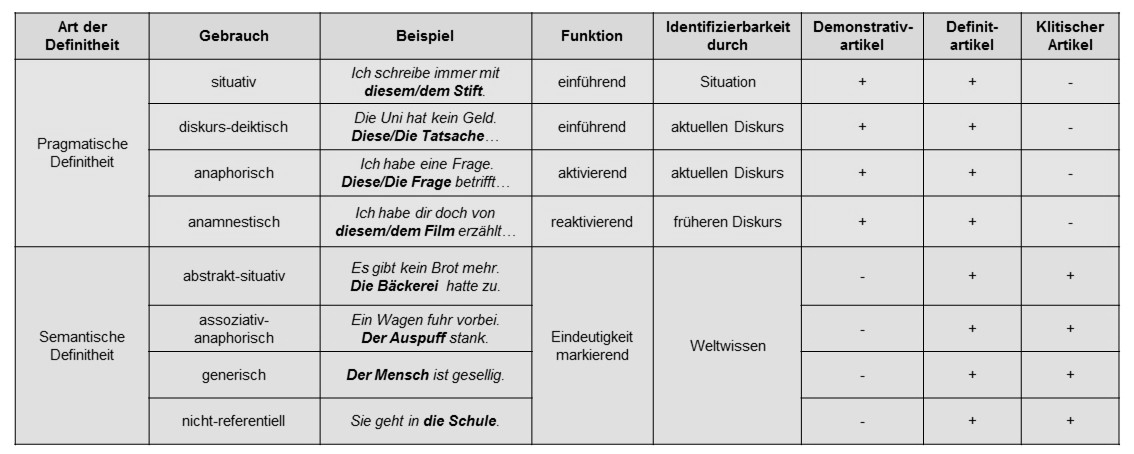
\includegraphics[width=12cm]{images/definit-kontexte-neu-sw.jpg}
\caption {Semantische und pragmatische Definita und ihre Gebrauchskontexte}
\label{abb:definita}
\end{center}
\end{figure}

Die empirische Relevanz der semantischen und pragmatischen Definitheit zeigt sich in Sprachen, die über zwei formal distinktive Artikelparadigmen verfügen -- bestehend aus einer unbetonten, reduzierten Form und einer betonten Vollform -- die den beiden Definitheitsarten entsprechen. Exemplarisch hierfür ist der von \textcite{Ebert1971} untersuchte  nordfriesische Dialekt Fering: Die phonologisch reduzierten A-Formen (\object{a/at}) sind den semantisch definiten Kontexten vorbehalten, während die vollen D-Formen (\object{di/det/dön}) nur in pragmatisch-definiten Kontexten vorkommen \parencite[529]{deMulder2011}.\footnote{Eine Übersicht zu weiteren ähnlichen Artikelsystemen gibt \textcite[]{Studler2011}. Die semantischen Unterschiede von starken und schwachen Definita werden -- vor dem Hintergrund formaler Definitheitstheorien -- ausführlich in \textcite{Schwarz2009} diskutiert.}

\textcite[112--117]{Demske2001} nutzt die Löbnersche Distinktion, um die Artikeldistribution im Althochdeutschen zu untersuchen. Sie argumentiert dafür, dass ahd. \object{dër}  auf pragmatische Definitheitskontexte beschränkt ist. Zur Illustration führt sie Belegstellen aus der ahd. Sprachperiode an, s. \xxref{ex:demske-prag1}{ex:demske-prag2}. 

\begin{exe} 
\ex \label{ex:demske-prag1}
	Situativer Gebrauch \\
	\gll \object{ther} \object{thaz} \object{uuort} \object{gihorit} \\
		Der dieses Wort hört\\
	\trans \extrans{Der dieses Wort hört} (T 75.3)
\end{exe}

\begin{exe} 
\ex \label{ex:demske-prag2} 
	Anaphorischer Gebrauch \\
	\gll \object{Ein} \object{búrg} \object{ist} \object{thar} \object{in} \object{lánte},...\object{zi} \object{theru} \object{steti} \\
		Eine Stadt ist dort im Land,...zu dieser Stadt...\\
	\trans  \extrans{Eine Stadt ist dort im Lande, ... zu dieser Stadt...} (O I 11,23--26)
\end{exe}

\noindent 
Hingegen bleiben in den gleichen Texten funktionale Konzepte, also semantische Definita \blockcquote[114]{Demske2001}{in der Regel} undeterminiert, s. \REF{ex:demske-sem1} und \REF{ex:demske-sem2}. 

\begin{exe} 
\ex \label{ex:demske-sem1} 
	Abstrakt-situativer Gebrauch: Unika \\
	\gll \object{Tho} \object{ward} \object{himil} \object{offan} \\
		Da ward Himmel offen \\
	\trans \extrans{Dann öffnete sich der Himmel} (O I,25,15) 
\end{exe}

\begin{exe} 
\ex \label{ex:demske-sem2} 
	Abstrakt-situativer Gebrauch: Superlative \\
	\gll \object{in} \object{ira} \object{bárm} \object{si} \object{sazta} \object{barno} \object{bézista}\\
		 in ihren Schoß sie setzte Kind liebstes\\
	\trans  \extrans{Sie setzte das liebste Kind in ihren Schoß} (O I 13,10)
\end{exe}

\noindent 
Die Belege suggerieren, dass das ahd. \object{dër} funktional dem heutigen Demonstrativartikel gleicht. Zu einem solchen Schluss kommt auch \textcite{Philippi1997}, die neben Beispielen aus dem Althochdeutschen auch Belege aus dem  Altsächsischen und Gotischen anführt: \blockcquote[86]{Philippi1997}{The distribution of definite determiners in the older Gmc [Germanic, JF] languages seems to be very similar to the distribution of demonstrative pronouns in the
modern Gmc languages}. 

Interessanterweise lassen sich aber auch Belege finden, die diesem Befund entgegenstehen: Nach \textcite{Kraiss2012} gibt es bspw. schon im ahd. Isidor NPs mit \object{dër} bei Superlativkonstruktionen, z.B: \object{mit dhem hohistom salidhorn} \extrans{mit der höchsten Seligkeit} (I 5,9). Auch Unika kommen in einigen Fällen schon mit \object{dër} vor \parencite[75]{Szczepaniak2011a}, z.B. \object{ther himil} \extrans{der Himmel} (O I,11). Zum generischen Gebrauch gibt es ebenfalls ganz unterschiedliche Beobachtungen. Kraiss geht nach seiner Durchsicht der größten althochdeutschen Textdenkmäler davon aus, dass weder im Isidor noch im Tatian generische Phrasen mit \object{dër} vorkommen. Seinen Analysen nach wird diese Expansionsstufe erst bei Otfrid beschritten \parencite[133]{Kraiss2012}. \textcite[80]{Oubouzar1992} spürt determinierte generische Referenzen allerdings schon im Tatian auf, s. \REF{ex:gen-tat-def}. Mit \object{ther man} liegt ein Fall von extensionaler Generizität vor; die Gattung Mensch wird verallgemeinert charakterisiert.  

\begin{exe} 
\ex \label{ex:gen-tat-def}
	\gll \object{nio} \object{mag} \object{\textbf{ther}} \object{\textbf{man}} \object{iouuiht} \object{intphahen}, \object{noba} \object{imo} \object{iz} \object{gigeban} \object{uuerde} \object{fon} \object{himile} \\
		Nie mag der Mensch irgendetwas empfangen, {wenn nicht} ihm es gegeben werde von Himmel\\
	\trans \extrans{Der Mensch kann nichts empfangen, wenn es
ihm nicht vom Himmel geschenkt werde} (T 21,5)
\end{exe}
\noindent 
\textcite{Petrova2020} verweist auf einen ähnlichen Beleg, den bereits \textcite[60]{Hodler1954} in den Monseer Fragmenten beschreibt. Hier hat die Phrase  \object{daer baum} eine  generische Lesart:  \object{So auh fona des baumes obaze · arcennit · uuir(dit) daer · baum}, nhd. sinngemäß: \extrans{Den Baum erkennt man an seiner Frucht} (M 6,15). 

Ferner sind Präposition-Artikel-Klisen ein weiteres wichtiges Indiz, dass \object{dër} bereits im Althochdeutschen in den Bereich der semantischen Definita eindringt. Sie kommen bereits im Tatian, vor allem aber bei Otfrid vor \parencite[vgl.][]{Nubling1992,Schlachter2015}, z.B. \object{zemo seuue Galileę} \extrans{zum See von Galiläe} oder \object{zen jungoron} \extrans{zu den Jüngern} (O 3, 23,27). 

Die Beispiele verdeutlichen, dass Aussagen zur Semantik und Expansion von \object{dër} nur schwer auf Basis von einzelnen, ausgewählten Belegstellen getroffen werden können. Um das Funk"-tions"-spektrum zu erfassen, muss erstens eine größere Menge an NPs mit und ohne \object{dër} analysiert werden. Zweitens ist es notwendig, transparente Analysekriterien zu schaffen, die durch ein theoretisches Modell begründet sind. In der vorliegenden Arbeit ist dies die Löbnersche Unterscheidung in pragmatische und semantische Definita und damit zusammenhängend die oben genannten Gebrauchskontexte für Demonstrativ- bzw. Definitartikel. Die Operationalisierung dieser Kriterien sowie die Auswahl der Belege wird im Methodenteil (Abschnitt \ref{sec:annotationsschritte}) erläutert. 

\section{Zusammenfassung}

In diesem Kapitel wurde das theoretische Gerüst vorgestellt, mit dem sich De"-mon"-stra"-tiv- von Definitartikeln funktional unterscheiden lassen. Es ist deutlich geworden, dass ein bestimmtes Grammem (hier: das ahd. \object{dër}) nur dann als Definitartikel klassifiziert werden kann, wenn es in semantisch-definiten Gebrauchskontexten \parencite{Lobner1985} erscheint. Dies sind Fälle, in denen der Referent unabhängig von der Gesprächssituation eindeutig identifizierbar ist, was  sowohl beim abstrakt-situativen (\object{Die Sonne scheint}) als auch beim assoziativ-anaphorischen Gebrauch (\object{\textbf{Die Lehne} an meinem Stuhl ist kaputt}) gegeben ist. Darüber hinaus wurden nicht-referentielle Gebrauchskontexte diskutiert, darunter generische Ausdrücke (\object{\textbf{Der Mensch} ist ein Säugetier}) und NPs mit nicht-spezifischen Referenten (\object{\textbf{zur Kirche} gehen}). Die Erkenntnisse aus der theoretischen Diskussion fließen in die Konzeption eines Annotationsleitfadens ein (s. \ref{sec:annotationsschritte}). Es wird davon ausgegangen, dass die Gebrauchskontexte nicht immer klar zu unterscheiden sind. Ambige Fälle zwischen pragmatischen, d.h. situationsabhängigen, und semantischen, also situationsunabhängigen Gebrauchskontexten sind besonders relevant, da sie Brückenkontexte für den kategorialen Wandel sein können. 
